\chapter{Εισαγωγή}

%Το \en{Lorem Ipsum} είναι απλά ένα κείμενο χωρίς νόημα για τους επαγγελματίες της τυπογραφίας και στοιχειοθεσίας \cite{LoremIpsumAll}. Το \en{Lorem Ipsum} είναι το επαγγελματικό πρότυπο όσον αφορά το κείμενο χωρίς νόημα, από τον 15ο αιώνα, όταν ένας ανώνυμος τυπογράφος πήρε ένα δοκίμιο και ανακάτεψε τις λέξεις για να δημιουργήσει ένα δείγμα βιβλίου. Όχι μόνο επιβίωσε πέντε αιώνες, αλλά κυριάρχησε στην ηλεκτρονική στοιχειοθεσία, παραμένοντας με κάθε τρόπο αναλλοίωτο. Έγινε δημοφιλές τη δεκαετία του '60 με την έκδοση των δειγμάτων της \en{Letraset} όπου περιελάμβαναν αποσπάσματα του \en{Lorem Ipsum}, και πιο πρόσφατα με το λογισμικό ηλεκτρονικής σελιδοποίησης όπως το \en{Aldus PageMaker} που περιείχαν εκδοχές του \en{Lorem Ipsum}.
Φαίνεται ότι ο χρόνος που σπαταλάνε οι μηχανικοί δικτύωσης όταν εισέρχονται σε εξοπλισμό δικτύωσης για να εισάγουν χειροκίνητα εντολές οπως για τη διαμόρφωση των συσκευών ή να εισέρχονται σε διακομιστές για τη χειροκίνητη
ρύθμιση μία προς μία μια λίστα συσκευών/δικτύων(\en{access lists}) είναι πολύ μεγάλος, συνεπώς η εποχή που όλα αυτά γινόντουσταν χειροκίνητα φτάνει στο τέλος της. Όλο και περισσότεροι/περισσότερες εταιρείες προωθούν την αυτοματοποίηση καθώς βλέπουν ότι κάθε
ώρα που επενδύεται στην αυτοματοποίηση μεταφράζεται σε πολλές ώρες εργασίας που εξοικονομούνται. 

Η αυτοματοποίηση αυτών των εργασιών με κάποια καλοφτιαγμένη λογική προγραμματισμού επιτρέπει
τη διαμόρφωση εκατοντάδων συσκευών μέσα σε λίγα λεπτά, απομακρύνει τη δυνατότητα
των λανθασμένων ρυθμίσεων που προέρχονται από ανθρώπινο λάθος, επιτρέπει την καταγραφή των αλλαγών διαμόρφωσης και έχει το πλεονέκτημα ότι καθιστά τη διαμόρφωση
τεχνικές λεπτομέρειες διαφανείς στον χρήστη που πρόκειται να ξεκινήσει τη διαδικασία αυτοματοποίησης. Για παράδειγμα, μια εταιρεία θα μπορούσε να αναθέσει υπεργολαβικά σε μια ομάδα λειτουργίας
που δεν έχει τεχνικές γνώσεις δικτύωσης και απλά παρέχοντάς τους μια
συγκεκριμένο σύνολο εισόδων θα μπορούσαν να διαμορφώσουν για Χ σημεία πρόσβασης σε Υ δίκτυα
ένα συγκεκριμένο SSID με τις επιθυμητές παραμέτρους. Οι δεδομένες είσοδοι θα μπορούσαν
να εισαχθούν από αυτούς σε μια εφαρμογή ιστού και ο υποκείμενος προγραμματισμός
κώδικας θα έκανε τα υπόλοιπα. Τελικά αυτό μεταφράζεται σε ένα πολύ γρήγορο και αξιόπιστο πλάνο κατά το οποίο η παραμετροποίηση και η
διαμόρφωση ενός δικτύου δεν θα χρειάζεται να γίνει από τους μηχανικούς δικτύωσης χειροκίνητα.

Μπορούν να επενδύσουν συνεπώς αυτόν τον επιπλέον χρόνο σε άλλες εργασίες όπως ο σχεδιασμός και έτσι οι πιο χρονοβόρες διαδικασίες να αυτοματοποιηθούν. Αλλά η αυτοματοποίηση δεν είναι μόνο
κάνει θαύματα όσον αφορά τη διαμόρφωση, είναι επίσης εξαιρετική για την παρακολούθηση της κατάστασης των δικτύων/συσκευών/θυρών, την απόκτηση πληροφοριών για την υγεία των ασύρματων δικτύων και κάθε
άλλες πληροφορίες που μπορούν να λάβουν από της δυκτυακές συσκευές.

Είναι σημαντικό να ληφθεί υπόψη ότι οι επαναλαμβανόμενες καθημερινές/εβδομαδιαίες εργασίες
που απαιτούν τη συλλογή πληροφοριών είναι εξαιρετικοί υποψήφιοι για αυτοματοποίηση.
Με μια αυτοματοποίηση που αναζητά τα απαιτούμενα δεδομένα και κάνει κάποια επεξεργασία οι απαιτούμενες πληροφορίες μπορούν να ληφθούν γρήγορα και να παρουσιαστούν στους
μηχανικό και τον/την απαλλάσσει από το να συνδέεται χειροκίνητα σε πολλές συσκευές, να ελέγχει
ορισμένων γραμμών διαμόρφωσης, κ.λπ.

Η αυτοματοποίηση συσκευών χρησιμοποιείται εδώ και πολλά χρόνια για τη διαχείριση βλαβών ή την παρακολούθηση του επιπέδου υπηρεσιών, αλλά με τις αυξανόμενες επιχειρηματικές ανάγκες προκύπτουν νέες προκλήσεις και νέες ευκαιρίες. 
Μία από αυτές τις ευκαιρίες είναι η επένδυση των εταιρειών σε αυτοματισμούς δικτύων.
Η ραγδαία ανάπτυξη των σύγχρονων δικτύων στις επιχειρήσεις μαζί με τις νέες τεχνολογίες, 
όπως το Διαδίκτυο των πραγμάτων (\en{IOT}) και το υπολογιστικό νέφος που βασίζονται επίσης στο δίκτυο, οδήγησαν στην ανάγκη ανάπτυξης της δικτυακής υποδομής με αποτέλεσμα την αύξηση του φόρτου εργασίας. 
απαιτήσεις για την παροχή, τη συντήρηση, την παρακολούθηση και τη διαχείριση από το δίκτυο. 

Οι μέθοδοι που χρησιμοποιούσαν μέχρι σήμερα οι μηχανικοί δικτύων δεν ήταν μόνο χρονοβόρες αλλά και 
απαιτούνταν και γνώσεις σχετικά με ιδιόκτητα πρωτόκολλα και τεχνολογίες.
Σε μια προσπάθεια να μειώσουν το κόστος και να δημιουργήσουν αποτελεσματικότητα οι μηχανικοί δικτύου ανέπτυξαν το \en{Network automation}
ως τεχνικές αυτοματοποίησης για την αυτοματοποίηση επαναλαμβανόμενων καθημερινών εργασιών.
Με την υποστήριξη σχεδόν όλων των μεγάλων εταιρειών δικτύωσης (όπως η \en{Cisco}) δημιουργήθηκε μια κοινότητα ανοιχτού κώδικα που είχε ως στόχο την υλοποίηση εφαρμογών αυτοματοποίησης 
κυρίως με τη χρήση τυποποιημένων διεπαφών (\en{SSH}, \en{REST}) και γενικών γλωσσών προγραμματισμού όπως η \en{python}.
Με τη χρήση της \en{Python} και μιας συλλογής ενοτήτων και συναρτήσεων θα προσπαθήσουμε να φτιάξουμε μία εφαρμογή που συνδέει όλα τα παραπάνω.


Παράλληλα η επανάσταση που έφερε η εισαγώγή της λογικής των \en{microservices} στον κλαδο της Πληροφορικής μπορεί να καθιστήσει την εφαρμογή αυτή ακόμα πιο αξιόπιστη
γιατί μπορεί να συμβάλει στο σχεδίασμό ενός συστήματος λογισμικού με μεγαλύτερη αξιοπιστία καθώς και να προσφέρει όλες εκείνες της θετικές προεκτάσεις χρήσης αυτών.
Θα γίνει λοιπόν μια προσπάθεια εισαγώγής τεχνολογιών διαχείρισης και ανάπτυξης \en{microservices} όπως \en{kubernetes} και \en{containers}. Τα πλεονεκτήματα της χρήσης της αρχιτεκτονική \en{Microservices} είναι ότι προσφέρουν μεγαλύτερη ευελιξία 
μέσω της ανεξαρτησίας των υπηρεσιών, επιτρέποντας στους οργανισμούς να γίνουν πιο ευέλικτοι όσον αφορά τον τρόπο με τον οποίο προσφέρουν νέες επιχειρηματικές δυνατότητες ή ανταποκρίνονται στις μεταβαλλόμενες συνθήκες της αγοράς. Αναλυτική παρουσίαση αυτών θα γίνει σε επόμενο κεφάλαιο. 

Σας συσκευές θα χρησιμοποιήσουμε αυτές της \en{Cisco} καθώς υπάρχουν ήδη βιβλιοθήκες οι οποίες υλοποιούν τα πρωτόκολλα επικοινωνίας και τις λειτουργίες που 
εμείς θέλουμε να υλοποιήσουμε. Η ανάπτυξη λογισμικού τέτοιων βιβλιοθηκών είναι αντικείμενο μελέτης διπλωματικής εργασίας καθώς ξεφεύγει από τα πλάισια μια μεταπτυχιακής διατριβής.

\section{Απαιτήσεις και προδιαγραφές}
\begin{itemize}
    \item \en{GNS3 VM} ,\en{Cisco} \en{Images} και \en{GNS3} περιβάλλον
    \item \en{Vs Code development environment}
    \item \en{Virtual box} ή οποιονδήποτε \en{type B hypervisor}
\end{itemize}

\section{Αυτοματοποίηση δικτύου}
Η αυτοματοποίηση του δικτύου δεν αφορά μόνο τη διαμόρφωση των συσκευών, αντίθετα, το πιο σημαντικό μέρος της αυτοματοποίησης δικτύου που συμβάλλει στη μείωση των ανθρώπινων σφαλμάτων είναι ότι δίνει στους
διαχειριστές τη δυνατότητα να αυτοματοποιούν διαδικασίες που εκτελούν τη συμμόρφωση και την επικύρωση  ελέγχους έναντι της τρέχουσας διαμόρφωσης ή οποιασδήποτε διαμόρφωσης που πρόκειται να αναπτυχθεί. 
Ως αποτέλεσμα, αυτό μειώνει τους χρόνους παράδοσης των αλλαγών στο δίκτυο και τον κίνδυνο διακοπής ή διανομής υπηρεσιών. Με αυτό τον τρόπο ελαχιστοποιεί επίσης την πιθανότητα ανθρώπινου λάθους και διασφαλίζει την ευθυγράμμιση με τις πολιτικές δικτύου.

Μια άλλη διαδικασία που μπορεί να αυτοματοποιηθεί είναι η αντιμετώπιση προβλημάτων. Όταν προκύπτει ένα πρόβλημα σε ένα 
το πρώτο βήμα για την επίλυση του προβλήματος είναι η συλλογή πληροφοριών. Η συλλογή των πληροφοριών από κάθε συσκευή μπορεί να είναι επίπονη και να απαιτεί πολύ χρόνο, ο οποίος είναι απαραίτητος, διότι συνήθως στο μεταξύ το δίκτυο, ή ένα τμήμα του, είναι εκτός λειτουργίας.
Χρησιμοποιώντας την αυτοματοποίηση δικτύου μπορούμε να αυτοματοποιήσουμε όλες τις εντολές που απαιτούνται για να λάβουμε τις πληροφορίες που απαιτούνται για την αντιμετώπιση προβλημάτων και να έχουμε πρόσβαση σε αυτές τις πληροφορίες σε πραγματικό χρόνο.
Η λήψη αυτών των πληροφοριών με προγραμματισμό σημαίνει ότι μπορούμε επίσης να τις ελέγξουμε σε  σε πραγματικό χρόνο. Ο έλεγχος των πληροφοριών σε πραγματικό χρόνο και η 
επιλογή των ενεργειών που πρέπει να ακολουθηθούν εάν κάποια από τις τιμές, για παράδειγμα η MTU, αλλάξουν, 
είναι μια τρίτη πτυχή της αυτοματοποίησης δικτύου που ονομάζεται αυτοματοποιημένη παρακολούθηση.
Η αυτοματοποιημένη παρακολούθηση συμβάλλει στην αποφυγή διακοπών που προκαλούνται από βλάβες υλικού.

Στην περίπτωση μας καθώς οι συσκευές είναι συσκευές με απλές λειτουργίες και δεν περιλαμβάνουν σύνθετα και πιο πολύπλοκα συστήματα κάποιες από τις λειτουργίες
που θα εκτελέσουμε είναι βασικές λειτουργίες που θα μπορούσαν να εκτελεστούν πολύ εύκολα και με χειροκίνητο τρόπο. Ένας από τους σκοπούς της διπλωματικής εργασίας
είναι να εξερευνήσει αυτές τις δυνατότητες.

\section{Τρόποι διαχείρησης δικτύου}
Για πολλά χρόνια το επίπεδο ελέγχου και το επίπεδο δεδομένων αναφέρονταν ως ένα στοιχείο ενός δικτύου. Στην περίπτωσή μας  





%\begin{equation}
%	y = \alpha x + \beta
%\end{equation}

%Αντίθετα με αυτό που θεωρεί η πλειοψηφία, το \en{Lorem Ipsum} δεν είναι απλά ένα τυχαίο κείμενο. Οι ρίζες του βρίσκονται σε ένα κείμενο Λατινικής λογοτεχνίας του 45 π.Χ., φτάνοντας την ηλικία του πάνω από 2000 έτη.


%\begin{figure}[htb]
%	\centering
%	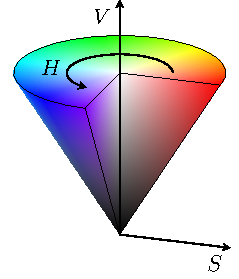
\includegraphics{tikz/hsv_cone/hsv_cone.pdf}
%	\caption{Ο χρωματικός χώρος \en{HSV}.}
%\end{figure}
